\documentclass{article}\usepackage[]{graphicx}\usepackage[]{xcolor}
% maxwidth is the original width if it is less than linewidth
% otherwise use linewidth (to make sure the graphics do not exceed the margin)
\makeatletter
\def\maxwidth{ %
  \ifdim\Gin@nat@width>\linewidth
    \linewidth
  \else
    \Gin@nat@width
  \fi
}
\makeatother

\definecolor{fgcolor}{rgb}{0.345, 0.345, 0.345}
\newcommand{\hlnum}[1]{\textcolor[rgb]{0.686,0.059,0.569}{#1}}%
\newcommand{\hlstr}[1]{\textcolor[rgb]{0.192,0.494,0.8}{#1}}%
\newcommand{\hlcom}[1]{\textcolor[rgb]{0.678,0.584,0.686}{\textit{#1}}}%
\newcommand{\hlopt}[1]{\textcolor[rgb]{0,0,0}{#1}}%
\newcommand{\hlstd}[1]{\textcolor[rgb]{0.345,0.345,0.345}{#1}}%
\newcommand{\hlkwa}[1]{\textcolor[rgb]{0.161,0.373,0.58}{\textbf{#1}}}%
\newcommand{\hlkwb}[1]{\textcolor[rgb]{0.69,0.353,0.396}{#1}}%
\newcommand{\hlkwc}[1]{\textcolor[rgb]{0.333,0.667,0.333}{#1}}%
\newcommand{\hlkwd}[1]{\textcolor[rgb]{0.737,0.353,0.396}{\textbf{#1}}}%
\let\hlipl\hlkwb

\usepackage{framed}
\makeatletter
\newenvironment{kframe}{%
 \def\at@end@of@kframe{}%
 \ifinner\ifhmode%
  \def\at@end@of@kframe{\end{minipage}}%
  \begin{minipage}{\columnwidth}%
 \fi\fi%
 \def\FrameCommand##1{\hskip\@totalleftmargin \hskip-\fboxsep
 \colorbox{shadecolor}{##1}\hskip-\fboxsep
     % There is no \\@totalrightmargin, so:
     \hskip-\linewidth \hskip-\@totalleftmargin \hskip\columnwidth}%
 \MakeFramed {\advance\hsize-\width
   \@totalleftmargin\z@ \linewidth\hsize
   \@setminipage}}%
 {\par\unskip\endMakeFramed%
 \at@end@of@kframe}
\makeatother

\definecolor{shadecolor}{rgb}{.97, .97, .97}
\definecolor{messagecolor}{rgb}{0, 0, 0}
\definecolor{warningcolor}{rgb}{1, 0, 1}
\definecolor{errorcolor}{rgb}{1, 0, 0}
\newenvironment{knitrout}{}{} % an empty environment to be redefined in TeX

\usepackage{alltt}
\usepackage[sc]{mathpazo}
\renewcommand{\sfdefault}{lmss}
\renewcommand{\ttdefault}{lmtt}
\usepackage[T1]{fontenc}
\usepackage{geometry}
\geometry{verbose,tmargin=2.5cm,bmargin=2.5cm,lmargin=2.5cm,rmargin=2.5cm}
\setcounter{secnumdepth}{2}
\setcounter{tocdepth}{2}
\usepackage[unicode=true,pdfusetitle,
 bookmarks=true,bookmarksnumbered=true,bookmarksopen=true,bookmarksopenlevel=2,
 breaklinks=false,pdfborder={0 0 1},backref=false,colorlinks=false]
 {hyperref}
\hypersetup{
 pdfstartview={XYZ null null 1}}

\makeatletter
%%%%%%%%%%%%%%%%%%%%%%%%%%%%%% User specified LaTeX commands.
\renewcommand{\textfraction}{0.05}
\renewcommand{\topfraction}{0.8}
\renewcommand{\bottomfraction}{0.8}
\renewcommand{\floatpagefraction}{0.75}

\makeatother
\IfFileExists{upquote.sty}{\usepackage{upquote}}{}
\begin{document}



\title{\title{\title{\title{\title{\title{\title{\title{\title{\title{\title{\title{}}}}}}}}}}}}



\maketitle
The results below are generated from an R script.

\begin{knitrout}
\definecolor{shadecolor}{rgb}{0.969, 0.969, 0.969}\color{fgcolor}\begin{kframe}
\begin{alltt}
\hlkwd{library}\hlstd{(ggplot2)}

\hlstd{df1}\hlkwb{=}\hlkwd{read.table}\hlstd{(}\hlstr{"./datos/student-mat.csv"}\hlstd{,}\hlkwc{sep}\hlstd{=}\hlstr{";"}\hlstd{,}\hlkwc{header}\hlstd{=}\hlnum{TRUE}\hlstd{)}
\hlstd{df2}\hlkwb{=}\hlkwd{read.table}\hlstd{(}\hlstr{"./datos/student-por.csv"}\hlstd{,}\hlkwc{sep}\hlstd{=}\hlstr{";"}\hlstd{,}\hlkwc{header}\hlstd{=}\hlnum{TRUE}\hlstd{)}

\hlstd{df3}\hlkwb{=}\hlkwd{merge}\hlstd{(df1,df2,}\hlkwc{by}\hlstd{=}\hlkwd{c}\hlstd{(}\hlstr{"school"}\hlstd{,}\hlstr{"sex"}\hlstd{,}\hlstr{"age"}\hlstd{,}\hlstr{"address"}\hlstd{,}\hlstr{"famsize"}\hlstd{,}\hlstr{"Pstatus"}\hlstd{,}\hlstr{"Medu"}\hlstd{,}\hlstr{"Fedu"}\hlstd{,}\hlstr{"Mjob"}\hlstd{,}\hlstr{"Fjob"}\hlstd{,}\hlstr{"reason"}\hlstd{,}\hlstr{"nursery"}\hlstd{,}\hlstr{"internet"}\hlstd{))}
\hlkwd{print}\hlstd{(}\hlkwd{nrow}\hlstd{(df3))} \hlcom{# 382 students}
\end{alltt}
\begin{verbatim}
## [1] 382
\end{verbatim}
\begin{alltt}
\hlcom{# Limpieza de datos}
\hlcom{# Resumen de datos}
\hlkwd{summary}\hlstd{(df3)}
\end{alltt}
\begin{verbatim}
##     school              sex                 age          address         
##  Length:382         Length:382         Min.   :15.00   Length:382        
##  Class :character   Class :character   1st Qu.:16.00   Class :character  
##  Mode  :character   Mode  :character   Median :17.00   Mode  :character  
##                                        Mean   :16.59                     
##                                        3rd Qu.:17.00                     
##                                        Max.   :22.00                     
##    famsize            Pstatus               Medu            Fedu           Mjob          
##  Length:382         Length:382         Min.   :0.000   Min.   :0.000   Length:382        
##  Class :character   Class :character   1st Qu.:2.000   1st Qu.:2.000   Class :character  
##  Mode  :character   Mode  :character   Median :3.000   Median :3.000   Mode  :character  
##                                        Mean   :2.806   Mean   :2.565                     
##                                        3rd Qu.:4.000   3rd Qu.:4.000                     
##                                        Max.   :4.000   Max.   :4.000                     
##      Fjob              reason            nursery            internet        
##  Length:382         Length:382         Length:382         Length:382        
##  Class :character   Class :character   Class :character   Class :character  
##  Mode  :character   Mode  :character   Mode  :character   Mode  :character  
##                                                                             
##                                                                             
##                                                                             
##   guardian.x         traveltime.x    studytime.x      failures.x     schoolsup.x       
##  Length:382         Min.   :1.000   Min.   :1.000   Min.   :0.0000   Length:382        
##  Class :character   1st Qu.:1.000   1st Qu.:1.000   1st Qu.:0.0000   Class :character  
##  Mode  :character   Median :1.000   Median :2.000   Median :0.0000   Mode  :character  
##                     Mean   :1.442   Mean   :2.034   Mean   :0.2906                     
##                     3rd Qu.:2.000   3rd Qu.:2.000   3rd Qu.:0.0000                     
##                     Max.   :4.000   Max.   :4.000   Max.   :3.0000                     
##    famsup.x            paid.x          activities.x         higher.x        
##  Length:382         Length:382         Length:382         Length:382        
##  Class :character   Class :character   Class :character   Class :character  
##  Mode  :character   Mode  :character   Mode  :character   Mode  :character  
##                                                                             
##                                                                             
##                                                                             
##   romantic.x           famrel.x      freetime.x       goout.x          Dalc.x     
##  Length:382         Min.   :1.00   Min.   :1.000   Min.   :1.000   Min.   :1.000  
##  Class :character   1st Qu.:4.00   1st Qu.:3.000   1st Qu.:2.000   1st Qu.:1.000  
##  Mode  :character   Median :4.00   Median :3.000   Median :3.000   Median :1.000  
##                     Mean   :3.94   Mean   :3.223   Mean   :3.113   Mean   :1.474  
##                     3rd Qu.:5.00   3rd Qu.:4.000   3rd Qu.:4.000   3rd Qu.:2.000  
##                     Max.   :5.00   Max.   :5.000   Max.   :5.000   Max.   :5.000  
##      Walc.x        health.x       absences.x          G1.x            G2.x      
##  Min.   :1.00   Min.   :1.000   Min.   : 0.000   Min.   : 3.00   Min.   : 0.00  
##  1st Qu.:1.00   1st Qu.:3.000   1st Qu.: 0.000   1st Qu.: 8.00   1st Qu.: 8.25  
##  Median :2.00   Median :4.000   Median : 3.000   Median :10.50   Median :11.00  
##  Mean   :2.28   Mean   :3.579   Mean   : 5.319   Mean   :10.86   Mean   :10.71  
##  3rd Qu.:3.00   3rd Qu.:5.000   3rd Qu.: 8.000   3rd Qu.:13.00   3rd Qu.:13.00  
##  Max.   :5.00   Max.   :5.000   Max.   :75.000   Max.   :19.00   Max.   :19.00  
##       G3.x        guardian.y         traveltime.y    studytime.y      failures.y    
##  Min.   : 0.00   Length:382         Min.   :1.000   Min.   :1.000   Min.   :0.0000  
##  1st Qu.: 8.00   Class :character   1st Qu.:1.000   1st Qu.:1.000   1st Qu.:0.0000  
##  Median :11.00   Mode  :character   Median :1.000   Median :2.000   Median :0.0000  
##  Mean   :10.39                      Mean   :1.445   Mean   :2.039   Mean   :0.1414  
##  3rd Qu.:14.00                      3rd Qu.:2.000   3rd Qu.:2.000   3rd Qu.:0.0000  
##  Max.   :20.00                      Max.   :4.000   Max.   :4.000   Max.   :3.0000  
##  schoolsup.y          famsup.y            paid.y          activities.y      
##  Length:382         Length:382         Length:382         Length:382        
##  Class :character   Class :character   Class :character   Class :character  
##  Mode  :character   Mode  :character   Mode  :character   Mode  :character  
##                                                                             
##                                                                             
##                                                                             
##    higher.y          romantic.y           famrel.y       freetime.y      goout.y     
##  Length:382         Length:382         Min.   :1.000   Min.   :1.00   Min.   :1.000  
##  Class :character   Class :character   1st Qu.:4.000   1st Qu.:3.00   1st Qu.:2.000  
##  Mode  :character   Mode  :character   Median :4.000   Median :3.00   Median :3.000  
##                                        Mean   :3.942   Mean   :3.23   Mean   :3.118  
##                                        3rd Qu.:5.000   3rd Qu.:4.00   3rd Qu.:4.000  
##                                        Max.   :5.000   Max.   :5.00   Max.   :5.000  
##      Dalc.y          Walc.y         health.y       absences.y          G1.y      
##  Min.   :1.000   Min.   :1.000   Min.   :1.000   Min.   : 0.000   Min.   : 0.00  
##  1st Qu.:1.000   1st Qu.:1.000   1st Qu.:3.000   1st Qu.: 0.000   1st Qu.:10.00  
##  Median :1.000   Median :2.000   Median :4.000   Median : 2.000   Median :12.00  
##  Mean   :1.476   Mean   :2.291   Mean   :3.576   Mean   : 3.673   Mean   :12.11  
##  3rd Qu.:2.000   3rd Qu.:3.000   3rd Qu.:5.000   3rd Qu.: 6.000   3rd Qu.:14.00  
##  Max.   :5.000   Max.   :5.000   Max.   :5.000   Max.   :32.000   Max.   :19.00  
##       G2.y            G3.y      
##  Min.   : 5.00   Min.   : 0.00  
##  1st Qu.:11.00   1st Qu.:11.00  
##  Median :12.00   Median :13.00  
##  Mean   :12.24   Mean   :12.52  
##  3rd Qu.:14.00   3rd Qu.:14.00  
##  Max.   :19.00   Max.   :19.00
\end{verbatim}
\begin{alltt}
\hlkwd{str}\hlstd{(df3)}
\end{alltt}
\begin{verbatim}
## 'data.frame':	382 obs. of  53 variables:
##  $ school      : chr  "GP" "GP" "GP" "GP" ...
##  $ sex         : chr  "F" "F" "F" "F" ...
##  $ age         : int  15 15 15 15 15 15 15 15 15 15 ...
##  $ address     : chr  "R" "R" "R" "R" ...
##  $ famsize     : chr  "GT3" "GT3" "GT3" "GT3" ...
##  $ Pstatus     : chr  "T" "T" "T" "T" ...
##  $ Medu        : int  1 1 2 2 3 3 3 2 3 3 ...
##  $ Fedu        : int  1 1 2 4 3 4 4 2 1 3 ...
##  $ Mjob        : chr  "at_home" "other" "at_home" "services" ...
##  $ Fjob        : chr  "other" "other" "other" "health" ...
##  $ reason      : chr  "home" "reputation" "reputation" "course" ...
##  $ nursery     : chr  "yes" "no" "yes" "yes" ...
##  $ internet    : chr  "yes" "yes" "no" "yes" ...
##  $ guardian.x  : chr  "mother" "mother" "mother" "mother" ...
##  $ traveltime.x: int  2 1 1 1 2 1 2 2 2 1 ...
##  $ studytime.x : int  4 2 1 3 3 3 3 2 4 4 ...
##  $ failures.x  : int  1 2 0 0 2 0 2 0 0 0 ...
##  $ schoolsup.x : chr  "yes" "yes" "yes" "yes" ...
##  $ famsup.x    : chr  "yes" "yes" "yes" "yes" ...
##  $ paid.x      : chr  "yes" "no" "yes" "yes" ...
##  $ activities.x: chr  "yes" "no" "yes" "yes" ...
##  $ higher.x    : chr  "yes" "yes" "yes" "yes" ...
##  $ romantic.x  : chr  "no" "yes" "no" "no" ...
##  $ famrel.x    : int  3 3 4 4 4 4 4 4 4 4 ...
##  $ freetime.x  : int  1 3 3 3 2 3 2 1 4 3 ...
##  $ goout.x     : int  2 4 1 2 1 2 2 3 2 3 ...
##  $ Dalc.x      : int  1 2 1 1 2 1 2 1 2 1 ...
##  $ Walc.x      : int  1 4 1 1 3 1 2 3 3 1 ...
##  $ health.x    : int  1 5 2 5 3 5 5 4 3 4 ...
##  $ absences.x  : int  2 2 8 2 8 2 0 2 12 10 ...
##  $ G1.x        : int  7 8 14 10 10 12 12 8 16 10 ...
##  $ G2.x        : int  10 6 13 9 10 12 0 9 16 11 ...
##  $ G3.x        : int  10 5 13 8 10 11 0 8 16 11 ...
##  $ guardian.y  : chr  "mother" "mother" "mother" "mother" ...
##  $ traveltime.y: int  2 1 1 1 2 1 2 2 2 1 ...
##  $ studytime.y : int  4 2 1 3 3 3 3 2 4 4 ...
##  $ failures.y  : int  0 0 0 0 0 0 0 0 0 0 ...
##  $ schoolsup.y : chr  "yes" "yes" "yes" "yes" ...
##  $ famsup.y    : chr  "yes" "yes" "yes" "yes" ...
##  $ paid.y      : chr  "yes" "no" "no" "no" ...
##  $ activities.y: chr  "yes" "no" "yes" "yes" ...
##  $ higher.y    : chr  "yes" "yes" "yes" "yes" ...
##  $ romantic.y  : chr  "no" "yes" "no" "no" ...
##  $ famrel.y    : int  3 3 4 4 4 4 4 4 4 4 ...
##  $ freetime.y  : int  1 3 3 3 2 3 2 1 4 3 ...
##  $ goout.y     : int  2 4 1 2 1 2 2 3 2 3 ...
##  $ Dalc.y      : int  1 2 1 1 2 1 2 1 2 1 ...
##  $ Walc.y      : int  1 4 1 1 3 1 2 3 3 1 ...
##  $ health.y    : int  1 5 2 5 3 5 5 4 3 4 ...
##  $ absences.y  : int  4 2 8 2 2 2 0 0 6 10 ...
##  $ G1.y        : int  13 13 14 10 13 11 10 11 15 10 ...
##  $ G2.y        : int  13 11 13 11 13 12 11 10 15 10 ...
##  $ G3.y        : int  13 11 12 10 13 12 12 11 15 10 ...
\end{verbatim}
\begin{alltt}
\hlcom{# Visualización de datos}
\hlstd{df3} \hlopt \hlkwd{ggplot}\hlstd{()} \hlopt{+}
  \hlkwd{geom_histogram}\hlstd{(}\hlkwc{mapping} \hlstd{=} \hlkwd{aes}\hlstd{(}\hlkwc{x} \hlstd{= G3.y))}
\end{alltt}


{\ttfamily\noindent\itshape\color{messagecolor}{\#\# `stat\_bin()` using `bins = 30`. Pick better value with `binwidth`.}}\end{kframe}

{\centering 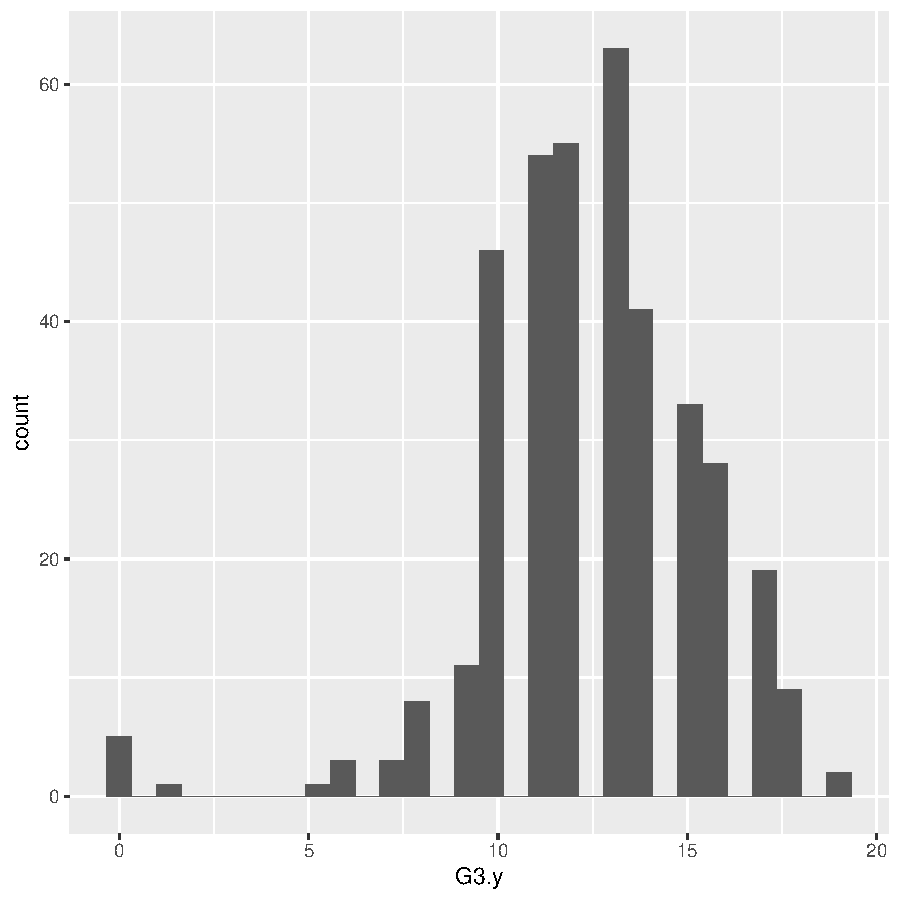
\includegraphics[width=.6\linewidth]{figure/LR1-SOLUCION-Rnwauto-report-1} 

}


\begin{kframe}\begin{alltt}
\hlcom{# nueva variable respuesta}
\hlstd{df3}\hlopt{$}\hlstd{final} \hlkwb{<-} \hlkwd{factor}\hlstd{(}\hlkwd{ifelse}\hlstd{(df3}\hlopt{$}\hlstd{G3.y} \hlopt{>=} \hlnum{10}\hlstd{,} \hlnum{1}\hlstd{,} \hlnum{0}\hlstd{),} \hlkwc{labels} \hlstd{=} \hlkwd{c}\hlstd{(}\hlstr{"fail"}\hlstd{,} \hlstr{"pass"}\hlstd{))}

\hlcom{# Fedu}
\hlkwd{ggplot}\hlstd{(df3,} \hlkwd{aes}\hlstd{(}\hlkwc{x}\hlstd{=Fedu,} \hlkwc{group}\hlstd{=final,}\hlkwc{fill}\hlstd{=final))} \hlopt{+} \hlkwd{geom_bar}\hlstd{()}
\end{alltt}
\end{kframe}

{\centering 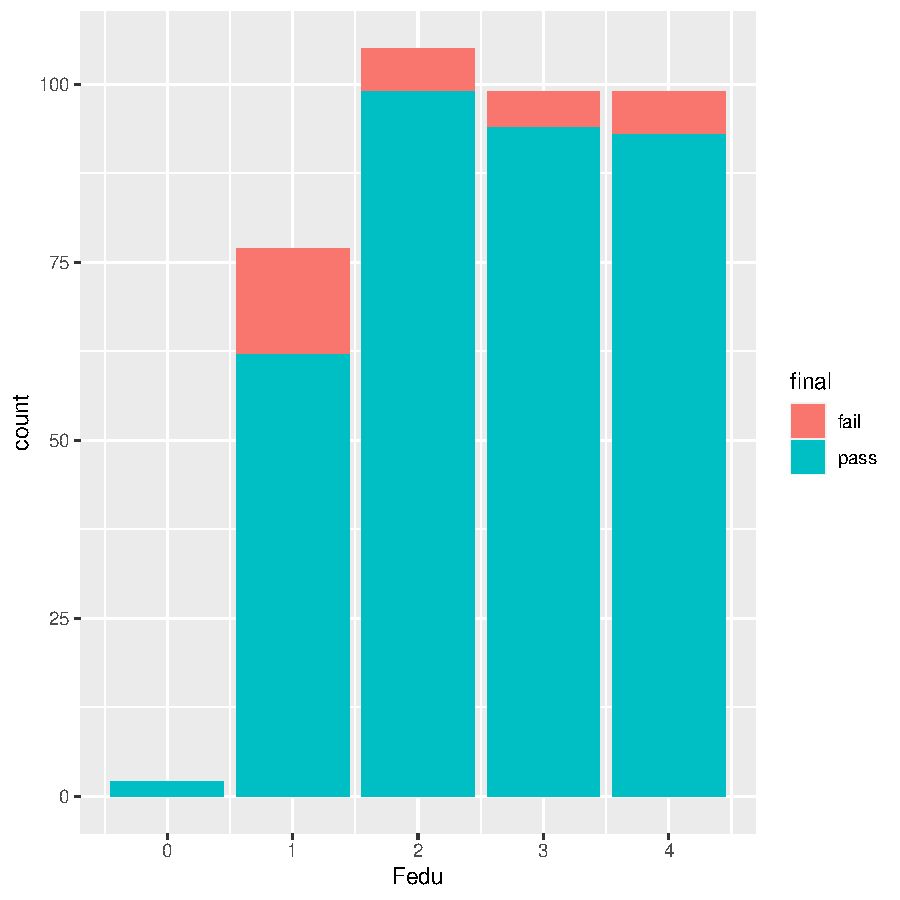
\includegraphics[width=.6\linewidth]{figure/LR1-SOLUCION-Rnwauto-report-2} 

}


\begin{kframe}\begin{alltt}
\hlcom{# Partición de datos}
\hlcom{# mediante una semilla conseguimos que el ejercicio sea reproducible}
\hlkwd{set.seed}\hlstd{(}\hlnum{1}\hlstd{)}

\hlcom{# Usamos el 70% de la base de datos como conjunto de entrenamiento y el resto como conjunto de test}
\hlstd{sample} \hlkwb{<-} \hlkwd{sample}\hlstd{(}\hlkwd{c}\hlstd{(}\hlnum{TRUE}\hlstd{,} \hlnum{FALSE}\hlstd{),} \hlkwd{nrow}\hlstd{(df3),} \hlkwc{replace}\hlstd{=}\hlnum{TRUE}\hlstd{,} \hlkwc{prob}\hlstd{=}\hlkwd{c}\hlstd{(}\hlnum{0.6}\hlstd{,}\hlnum{0.4}\hlstd{))}
\hlstd{datos.train}  \hlkwb{<-} \hlstd{df3[sample, ]}
\hlstd{datos.test}   \hlkwb{<-} \hlstd{df3[}\hlopt{!}\hlstd{sample, ]}

\hlkwd{dim}\hlstd{(datos.train)}
\end{alltt}
\begin{verbatim}
## [1] 241  54
\end{verbatim}
\begin{alltt}
\hlstd{lr1} \hlkwb{<-} \hlkwd{glm}\hlstd{(final} \hlopt{~} \hlstd{Fedu ,} \hlkwc{data}\hlstd{= datos.train,}\hlkwc{family}\hlstd{=binomial)}
\hlkwd{summary}\hlstd{(lr1)}
\end{alltt}
\begin{verbatim}
## 
## Call:
## glm(formula = final ~ Fedu, family = binomial, data = datos.train)
## 
## Coefficients:
##             Estimate Std. Error z value Pr(>|z|)   
## (Intercept)   0.8617     0.5189   1.661  0.09679 . 
## Fedu          0.6938     0.2405   2.885  0.00391 **
## ---
## Signif. codes:  0 '***' 0.001 '**' 0.01 '*' 0.05 '.' 0.1 ' ' 1
## 
## (Dispersion parameter for binomial family taken to be 1)
## 
##     Null deviance: 137.85  on 240  degrees of freedom
## Residual deviance: 128.51  on 239  degrees of freedom
## AIC: 132.51
## 
## Number of Fisher Scoring iterations: 6
\end{verbatim}
\begin{alltt}
\hlstd{lr1} \hlkwb{<-} \hlkwd{glm}\hlstd{(final} \hlopt{~} \hlkwd{as.factor}\hlstd{(Fedu) ,} \hlkwc{data}\hlstd{= datos.train,}\hlkwc{family}\hlstd{=binomial)}
\hlkwd{summary}\hlstd{(lr1)}
\end{alltt}
\begin{verbatim}
## 
## Call:
## glm(formula = final ~ as.factor(Fedu), family = binomial, data = datos.train)
## 
## Coefficients:
##                  Estimate Std. Error z value Pr(>|z|)
## (Intercept)         15.57    1029.12   0.015    0.988
## as.factor(Fedu)1   -14.38    1029.12  -0.014    0.989
## as.factor(Fedu)2   -12.83    1029.12  -0.012    0.990
## as.factor(Fedu)3   -12.05    1029.12  -0.012    0.991
## as.factor(Fedu)4   -12.68    1029.12  -0.012    0.990
## 
## (Dispersion parameter for binomial family taken to be 1)
## 
##     Null deviance: 137.85  on 240  degrees of freedom
## Residual deviance: 122.94  on 236  degrees of freedom
## AIC: 132.94
## 
## Number of Fisher Scoring iterations: 14
\end{verbatim}
\begin{alltt}
\hlcom{# Reagrupamos }
\hlstd{datos.train}\hlkwb{=}
  \hlstd{datos.train} \hlopt
  \hlkwd{mutate}\hlstd{(}\hlkwc{Fedu_bin}\hlstd{=}\hlkwd{as.factor}\hlstd{(}\hlkwd{ifelse}\hlstd{(Fedu}\hlopt{>}\hlnum{1}\hlstd{,}\hlnum{1}\hlstd{,}\hlnum{0}\hlstd{)))}

\hlstd{lr1} \hlkwb{<-} \hlkwd{glm}\hlstd{(final} \hlopt{~} \hlstd{Fedu_bin ,} \hlkwc{data}\hlstd{= datos.train,}\hlkwc{family}\hlstd{=binomial)}
\hlkwd{summary}\hlstd{(lr1)}
\end{alltt}
\begin{verbatim}
## 
## Call:
## glm(formula = final ~ Fedu_bin, family = binomial, data = datos.train)
## 
## Coefficients:
##             Estimate Std. Error z value Pr(>|z|)    
## (Intercept)   1.2397     0.3424   3.621 0.000294 ***
## Fedu_bin1     1.7726     0.4835   3.666 0.000246 ***
## ---
## Signif. codes:  0 '***' 0.001 '**' 0.01 '*' 0.05 '.' 0.1 ' ' 1
## 
## (Dispersion parameter for binomial family taken to be 1)
## 
##     Null deviance: 137.85  on 240  degrees of freedom
## Residual deviance: 124.84  on 239  degrees of freedom
## AIC: 128.84
## 
## Number of Fisher Scoring iterations: 5
\end{verbatim}
\begin{alltt}
\hlkwd{ggplot}\hlstd{(datos.train,} \hlkwd{aes}\hlstd{(}\hlkwc{x}\hlstd{=Fedu_bin,} \hlkwc{group}\hlstd{=final,}\hlkwc{fill}\hlstd{=final))} \hlopt{+} \hlkwd{geom_bar}\hlstd{()}
\end{alltt}
\end{kframe}

{\centering 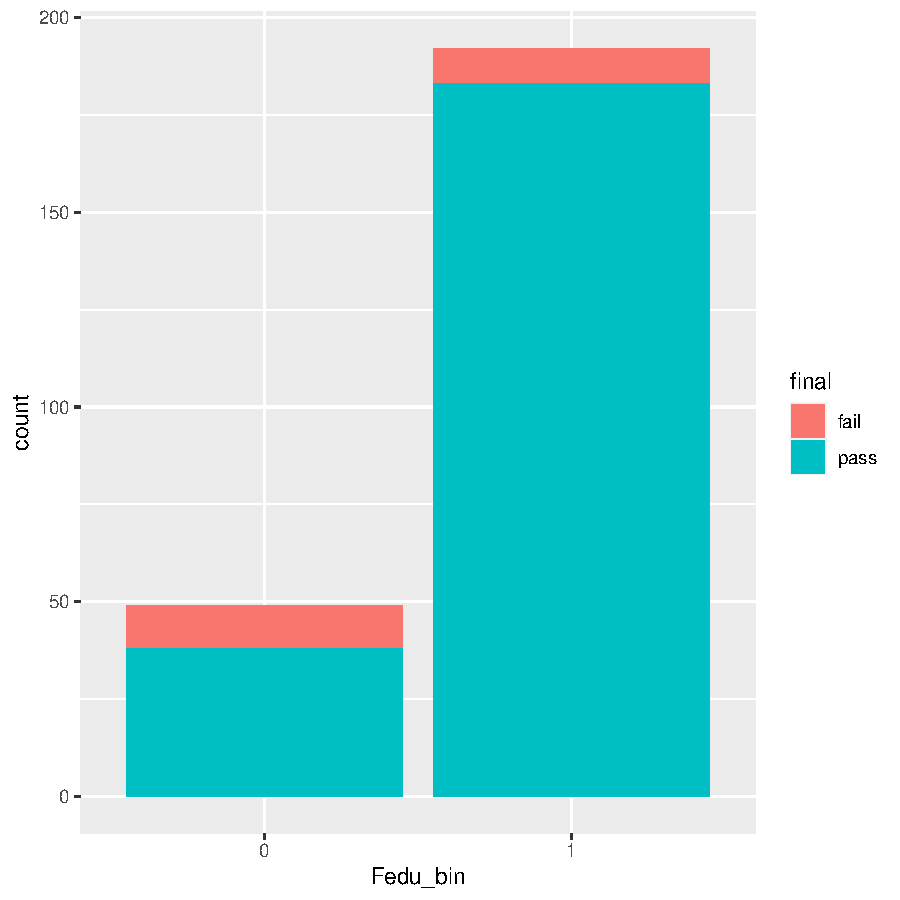
\includegraphics[width=.6\linewidth]{figure/LR1-SOLUCION-Rnwauto-report-3} 

}


\begin{kframe}\begin{alltt}
\hlcom{# Medu}

\hlstd{lr1} \hlkwb{<-} \hlkwd{glm}\hlstd{(final} \hlopt{~} \hlstd{Medu ,} \hlkwc{data}\hlstd{= datos.train,}\hlkwc{family}\hlstd{=binomial)}
\hlkwd{summary}\hlstd{(lr1)}
\end{alltt}
\begin{verbatim}
## 
## Call:
## glm(formula = final ~ Medu, family = binomial, data = datos.train)
## 
## Coefficients:
##             Estimate Std. Error z value Pr(>|z|)  
## (Intercept)   1.1114     0.5649   1.967   0.0492 *
## Medu          0.5079     0.2227   2.281   0.0226 *
## ---
## Signif. codes:  0 '***' 0.001 '**' 0.01 '*' 0.05 '.' 0.1 ' ' 1
## 
## (Dispersion parameter for binomial family taken to be 1)
## 
##     Null deviance: 137.85  on 240  degrees of freedom
## Residual deviance: 132.45  on 239  degrees of freedom
## AIC: 136.45
## 
## Number of Fisher Scoring iterations: 5
\end{verbatim}
\begin{alltt}
\hlstd{lr1} \hlkwb{<-} \hlkwd{glm}\hlstd{(final} \hlopt{~} \hlkwd{as.factor}\hlstd{(Medu) ,} \hlkwc{data}\hlstd{= datos.train,}\hlkwc{family}\hlstd{=binomial)}
\hlkwd{summary}\hlstd{(lr1)}
\end{alltt}
\begin{verbatim}
## 
## Call:
## glm(formula = final ~ as.factor(Medu), family = binomial, data = datos.train)
## 
## Coefficients:
##                  Estimate Std. Error z value Pr(>|z|)
## (Intercept)         15.57    1455.40   0.011    0.991
## as.factor(Medu)1   -14.10    1455.40  -0.010    0.992
## as.factor(Medu)2   -13.26    1455.40  -0.009    0.993
## as.factor(Medu)3   -13.15    1455.40  -0.009    0.993
## as.factor(Medu)4   -12.31    1455.40  -0.008    0.993
## 
## (Dispersion parameter for binomial family taken to be 1)
## 
##     Null deviance: 137.85  on 240  degrees of freedom
## Residual deviance: 131.35  on 236  degrees of freedom
## AIC: 141.35
## 
## Number of Fisher Scoring iterations: 14
\end{verbatim}
\begin{alltt}
\hlcom{# Aquí podríamos agrupar, o no. Agrupamos y estudiamos qué ocurre.}

\hlcom{# Reagrupamos }
\hlstd{datos.train}\hlkwb{=}
  \hlstd{datos.train} \hlopt
  \hlkwd{mutate}\hlstd{(}\hlkwc{Medu_bin}\hlstd{=}\hlkwd{as.factor}\hlstd{(}\hlkwd{ifelse}\hlstd{(Medu}\hlopt{>}\hlnum{1}\hlstd{,}\hlnum{1}\hlstd{,}\hlnum{0}\hlstd{)))}

\hlstd{lr1} \hlkwb{<-} \hlkwd{glm}\hlstd{(final} \hlopt{~} \hlstd{Medu_bin ,} \hlkwc{data}\hlstd{= datos.train,}\hlkwc{family}\hlstd{=binomial)}
\hlkwd{summary}\hlstd{(lr1)}
\end{alltt}
\begin{verbatim}
## 
## Call:
## glm(formula = final ~ Medu_bin, family = binomial, data = datos.train)
## 
## Coefficients:
##             Estimate Std. Error z value Pr(>|z|)    
## (Intercept)   1.5041     0.4513   3.333 0.000861 ***
## Medu_bin1     1.1247     0.5294   2.124 0.033633 *  
## ---
## Signif. codes:  0 '***' 0.001 '**' 0.01 '*' 0.05 '.' 0.1 ' ' 1
## 
## (Dispersion parameter for binomial family taken to be 1)
## 
##     Null deviance: 137.85  on 240  degrees of freedom
## Residual deviance: 133.89  on 239  degrees of freedom
## AIC: 137.89
## 
## Number of Fisher Scoring iterations: 5
\end{verbatim}
\begin{alltt}
\hlkwd{ggplot}\hlstd{(datos.train,} \hlkwd{aes}\hlstd{(}\hlkwc{x}\hlstd{=Fedu_bin,} \hlkwc{group}\hlstd{=final,}\hlkwc{fill}\hlstd{=final))} \hlopt{+} \hlkwd{geom_bar}\hlstd{()}
\end{alltt}
\end{kframe}

{\centering 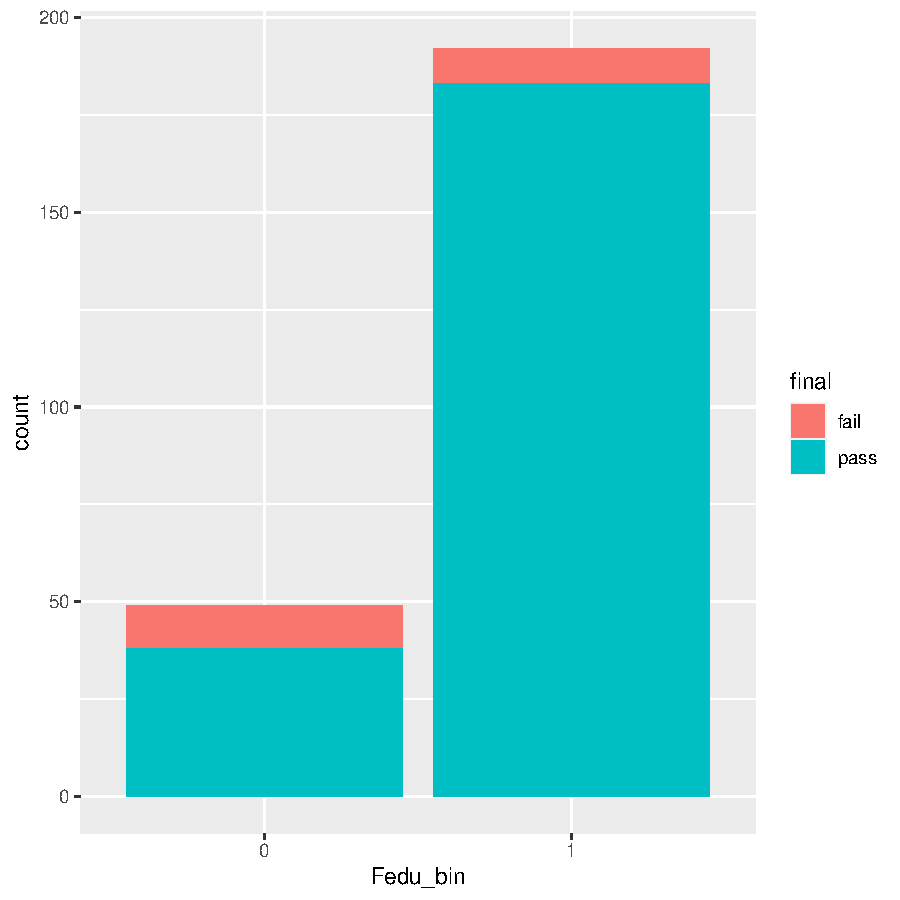
\includegraphics[width=.6\linewidth]{figure/LR1-SOLUCION-Rnwauto-report-4} 

}


\begin{kframe}\begin{alltt}
\hlcom{# En este caso, se pierde significatividad estadística y se decide no agrupar con las mismas categorías que Fedu, }
\hlcom{# sino como sigue:}
\hlstd{datos.train}\hlkwb{=}
  \hlstd{datos.train} \hlopt
  \hlkwd{mutate}\hlstd{(}\hlkwc{Medu_bin}\hlstd{=}\hlkwd{as.factor}\hlstd{(}\hlkwd{ifelse}\hlstd{(Medu}\hlopt{==}\hlnum{4}\hlstd{,}\hlnum{1}\hlstd{,}\hlnum{0}\hlstd{)))}

\hlstd{lr1} \hlkwb{<-} \hlkwd{glm}\hlstd{(final} \hlopt{~} \hlstd{Medu_bin ,} \hlkwc{data}\hlstd{= datos.train,}\hlkwc{family}\hlstd{=binomial)}
\hlkwd{summary}\hlstd{(lr1)}
\end{alltt}
\begin{verbatim}
## 
## Call:
## glm(formula = final ~ Medu_bin, family = binomial, data = datos.train)
## 
## Coefficients:
##             Estimate Std. Error z value Pr(>|z|)    
## (Intercept)   2.1296     0.2565   8.301   <2e-16 ***
## Medu_bin1     1.1285     0.6418   1.758   0.0787 .  
## ---
## Signif. codes:  0 '***' 0.001 '**' 0.01 '*' 0.05 '.' 0.1 ' ' 1
## 
## (Dispersion parameter for binomial family taken to be 1)
## 
##     Null deviance: 137.85  on 240  degrees of freedom
## Residual deviance: 134.02  on 239  degrees of freedom
## AIC: 138.02
## 
## Number of Fisher Scoring iterations: 6
\end{verbatim}
\begin{alltt}
\hlcom{# LR}

\hlstd{lr1} \hlkwb{<-} \hlkwd{glm}\hlstd{(final} \hlopt{~} \hlstd{Fedu_bin}\hlopt{+}\hlstd{Medu_bin,} \hlkwc{data}\hlstd{= datos.train,}\hlkwc{family}\hlstd{=binomial)}
\hlkwd{summary}\hlstd{(lr1)}
\end{alltt}
\begin{verbatim}
## 
## Call:
## glm(formula = final ~ Fedu_bin + Medu_bin, family = binomial, 
##     data = datos.train)
## 
## Coefficients:
##             Estimate Std. Error z value Pr(>|z|)    
## (Intercept)   1.2315     0.3427   3.594 0.000326 ***
## Fedu_bin1     1.6130     0.5299   3.044 0.002333 ** 
## Medu_bin1     0.4561     0.7082   0.644 0.519549    
## ---
## Signif. codes:  0 '***' 0.001 '**' 0.01 '*' 0.05 '.' 0.1 ' ' 1
## 
## (Dispersion parameter for binomial family taken to be 1)
## 
##     Null deviance: 137.85  on 240  degrees of freedom
## Residual deviance: 124.41  on 238  degrees of freedom
## AIC: 130.41
## 
## Number of Fisher Scoring iterations: 6
\end{verbatim}
\begin{alltt}
\hlcom{# Modelo básico}
\hlstd{base.mod} \hlkwb{<-} \hlkwd{glm}\hlstd{(final} \hlopt{~} \hlnum{1} \hlstd{,} \hlkwc{data}\hlstd{= datos.train,}\hlkwc{family}\hlstd{=binomial)}

\hlcom{# Modelo completo}
\hlstd{all.mod} \hlkwb{<-} \hlkwd{glm}\hlstd{(final} \hlopt{~} \hlstd{Fedu_bin}\hlopt{+}\hlstd{Medu_bin}\hlopt{+}\hlstd{age}\hlopt{+}\hlstd{sex}\hlopt{+}\hlstd{school}\hlopt{+}\hlstd{famsize}\hlopt{+}\hlstd{Mjob}\hlopt{+}\hlstd{Fjob}\hlopt{+}\hlstd{reason ,} \hlkwc{data}\hlstd{= datos.train,}\hlkwc{family}\hlstd{=binomial)}

\hlcom{# Step-wise}
\hlstd{stepMod} \hlkwb{<-} \hlkwd{step}\hlstd{(base.mod,} \hlkwc{scope} \hlstd{=} \hlkwd{list}\hlstd{(}\hlkwc{lower} \hlstd{= base.mod,} \hlkwc{upper} \hlstd{= all.mod),} \hlkwc{direction} \hlstd{=} \hlstr{"both"}\hlstd{,} \hlkwc{trace} \hlstd{=} \hlnum{0}\hlstd{,} \hlkwc{steps} \hlstd{=} \hlnum{1000}\hlstd{)}

\hlcom{# Variables en el modelo}
\hlkwd{formula}\hlstd{(stepMod)}
\end{alltt}
\begin{verbatim}
## final ~ Fedu_bin + sex + school
\end{verbatim}
\begin{alltt}
\hlcom{# Construcción del modelo}
\hlkwd{set.seed}\hlstd{(}\hlnum{1337}\hlstd{)}

\hlcom{#  10-fold cross validation}
\hlstd{train_control} \hlkwb{<-} \hlkwd{trainControl}\hlstd{(}\hlkwc{method}\hlstd{=}\hlstr{"cv"}\hlstd{,} \hlkwc{number}\hlstd{=}\hlnum{10}\hlstd{)}

\hlcom{# Entrenamos el modelo empleando glm }
\hlstd{model} \hlkwb{<-} \hlkwd{train}\hlstd{(}\hlkwd{formula}\hlstd{(stepMod),} \hlkwc{data} \hlstd{= datos.train,} \hlkwc{method} \hlstd{=} \hlstr{"glm"}\hlstd{,}\hlkwc{trControl}\hlstd{=train_control,}\hlkwc{family} \hlstd{= binomial)}

\hlcom{# Resumen del modelo}
\hlkwd{summary}\hlstd{(model)}
\end{alltt}
\begin{verbatim}
## 
## Call:
## NULL
## 
## Coefficients:
##             Estimate Std. Error z value Pr(>|z|)    
## (Intercept)   2.4959     0.5815   4.292 1.77e-05 ***
## Fedu_bin1     1.6921     0.5135   3.295 0.000984 ***
## sexM         -1.4388     0.5751  -2.502 0.012360 *  
## schoolMS     -1.5843     0.5832  -2.717 0.006597 ** 
## ---
## Signif. codes:  0 '***' 0.001 '**' 0.01 '*' 0.05 '.' 0.1 ' ' 1
## 
## (Dispersion parameter for binomial family taken to be 1)
## 
##     Null deviance: 137.85  on 240  degrees of freedom
## Residual deviance: 111.62  on 237  degrees of freedom
## AIC: 119.62
## 
## Number of Fisher Scoring iterations: 6
\end{verbatim}
\begin{alltt}
\hlcom{# Evaluación del modelo}
\hlstd{datos.test}\hlkwb{=}
  \hlstd{datos.test} \hlopt
  \hlkwd{mutate}\hlstd{(}\hlkwc{Fedu_bin}\hlstd{=}\hlkwd{as.factor}\hlstd{(}\hlkwd{ifelse}\hlstd{(Fedu}\hlopt{>}\hlnum{1}\hlstd{,}\hlnum{1}\hlstd{,}\hlnum{0}\hlstd{)),} \hlkwc{Medu_bin}\hlstd{=}\hlkwd{as.factor}\hlstd{(}\hlkwd{ifelse}\hlstd{(Medu}\hlopt{==}\hlnum{4}\hlstd{,}\hlnum{1}\hlstd{,}\hlnum{0}\hlstd{)))}


\hlstd{prediction} \hlkwb{<-} \hlkwd{predict}\hlstd{(model,} \hlkwc{newdata} \hlstd{= datos.test,} \hlkwc{type} \hlstd{=} \hlstr{"raw"}\hlstd{)}
\hlkwd{confusionMatrix}\hlstd{(}\hlkwd{table}\hlstd{(prediction, datos.test}\hlopt{$}\hlstd{final),} \hlkwc{positive} \hlstd{=} \hlstr{"pass"}\hlstd{)}
\end{alltt}
\begin{verbatim}
## Confusion Matrix and Statistics
## 
##           
## prediction fail pass
##       fail    0    1
##       pass   12  128
##                                         
##                Accuracy : 0.9078        
##                  95% CI : (0.8475, 0.95)
##     No Information Rate : 0.9149        
##     P-Value [Acc > NIR] : 0.686406      
##                                         
##                   Kappa : -0.0133       
##                                         
##  Mcnemar's Test P-Value : 0.005546      
##                                         
##             Sensitivity : 0.9922        
##             Specificity : 0.0000        
##          Pos Pred Value : 0.9143        
##          Neg Pred Value : 0.0000        
##              Prevalence : 0.9149        
##          Detection Rate : 0.9078        
##    Detection Prevalence : 0.9929        
##       Balanced Accuracy : 0.4961        
##                                         
##        'Positive' Class : pass          
## 
\end{verbatim}
\end{kframe}
\end{knitrout}

The R session information (including the OS info, R version and all
packages used):

\begin{knitrout}
\definecolor{shadecolor}{rgb}{0.969, 0.969, 0.969}\color{fgcolor}\begin{kframe}
\begin{alltt}
\hlkwd{sessionInfo}\hlstd{()}
\end{alltt}
\begin{verbatim}
## R version 4.3.1 (2023-06-16)
## Platform: x86_64-pc-linux-gnu (64-bit)
## Running under: Ubuntu 20.04.6 LTS
## 
## Matrix products: default
## BLAS:   /usr/lib/x86_64-linux-gnu/atlas/libblas.so.3.10.3 
## LAPACK: /usr/lib/x86_64-linux-gnu/atlas/liblapack.so.3.10.3;  LAPACK version 3.9.0
## 
## locale:
##  [1] LC_CTYPE=es_ES.UTF-8       LC_NUMERIC=C               LC_TIME=es_ES.UTF-8       
##  [4] LC_COLLATE=es_ES.UTF-8     LC_MONETARY=es_ES.UTF-8    LC_MESSAGES=es_ES.UTF-8   
##  [7] LC_PAPER=es_ES.UTF-8       LC_NAME=C                  LC_ADDRESS=C              
## [10] LC_TELEPHONE=C             LC_MEASUREMENT=es_ES.UTF-8 LC_IDENTIFICATION=C       
## 
## time zone: Europe/Madrid
## tzcode source: system (glibc)
## 
## attached base packages:
## [1] grid      stats     graphics  grDevices utils     datasets  methods   base     
## 
## other attached packages:
##  [1] randomForestExplainer_0.10.1 partykit_1.2-20             
##  [3] mvtnorm_1.2-3                libcoin_1.0-10              
##  [5] blorr_0.3.0                  Hmisc_5.1-1                 
##  [7] readr_2.1.4                  caretEnsemble_2.0.3         
##  [9] DALEX_2.4.3                  ROCR_1.0-11                 
## [11] randomForest_4.7-1.1         arulesViz_1.5-2             
## [13] arules_1.7-6                 Matrix_1.6-1.1              
## [15] liver_1.15                   ggfortify_0.4.16            
## [17] factoextra_1.0.7             mlbench_2.1-3.1             
## [19] readxl_1.4.3                 caret_6.0-94                
## [21] lattice_0.21-9               ggplot2_3.4.3               
## [23] rpart.plot_3.1.1             rpart_4.1.19                
## [25] caTools_1.18.2               dplyr_1.1.3                 
## [27] ISLR2_1.3-2                 
## 
## loaded via a namespace (and not attached):
##   [1] RColorBrewer_1.1-3   rstudioapi_0.15.0    jsonlite_1.8.7       magrittr_2.0.3      
##   [5] farver_2.1.1         rmarkdown_2.25       vctrs_0.6.3          base64enc_0.1-3     
##   [9] iBreakDown_2.0.1     tinytex_0.47         htmltools_0.5.6.1    cellranger_1.1.0    
##  [13] Formula_1.2-5        pROC_1.18.4          parallelly_1.36.0    htmlwidgets_1.6.2   
##  [17] plyr_1.8.9           lubridate_1.9.3      igraph_1.5.1         lifecycle_1.0.3     
##  [21] iterators_1.0.14     pkgconfig_2.0.3      R6_2.5.1             fastmap_1.1.1       
##  [25] future_1.33.0        digest_0.6.33        reshape_0.8.9        GGally_2.1.2        
##  [29] colorspace_2.1-0     labeling_0.4.3       fansi_1.0.5          timechange_0.2.0    
##  [33] abind_1.4-5          polyclip_1.10-6      compiler_4.3.1       proxy_0.4-27        
##  [37] bit64_4.0.5          withr_2.5.1          htmlTable_2.4.1      backports_1.4.1     
##  [41] carData_3.0-5        viridis_0.6.4        highr_0.10           ggforce_0.4.1       
##  [45] MASS_7.3-60          lava_1.7.2.1         ModelMetrics_1.2.2.2 tools_4.3.1         
##  [49] foreign_0.8-85       future.apply_1.11.0  nnet_7.3-19          glue_1.6.2          
##  [53] inum_1.0-5           nlme_3.1-163         checkmate_2.2.0      cluster_2.1.4       
##  [57] reshape2_1.4.4       generics_0.1.3       recipes_1.0.8        gtable_0.3.4        
##  [61] tzdb_0.4.0           class_7.3-22         tidyr_1.3.0          data.table_1.14.8   
##  [65] hms_1.1.3            car_3.1-2            tidygraph_1.2.3      utf8_1.2.3          
##  [69] ggrepel_0.9.3        foreach_1.5.2        pillar_1.9.0         stringr_1.5.0       
##  [73] vroom_1.6.4          splines_4.3.1        tweenr_2.0.2         survival_3.5-7      
##  [77] bit_4.0.5            tidyselect_1.2.0     pbapply_1.7-2        knitr_1.44          
##  [81] gridExtra_2.3        stats4_4.3.1         xfun_0.40            graphlayouts_1.0.1  
##  [85] hardhat_1.3.0        timeDate_4022.108    DT_0.30              visNetwork_2.1.2    
##  [89] stringi_1.7.12       yaml_2.3.7           evaluate_0.22        codetools_0.2-19    
##  [93] ggraph_2.1.0         tibble_3.2.1         cli_3.6.1            munsell_0.5.0       
##  [97] Rcpp_1.0.11          globals_0.16.2       parallel_4.3.1       ellipsis_0.3.2      
## [101] gower_1.0.1          bitops_1.0-7         listenv_0.9.0        viridisLite_0.4.2   
## [105] ipred_0.9-14         scales_1.2.1         prodlim_2023.08.28   e1071_1.7-13        
## [109] purrr_1.0.2          crayon_1.5.2         rlang_1.1.1
\end{verbatim}
\begin{alltt}
\hlkwd{Sys.time}\hlstd{()}
\end{alltt}
\begin{verbatim}
## [1] "2023-11-03 11:55:32 CET"
\end{verbatim}
\end{kframe}
\end{knitrout}


\end{document}
